\section{Method}
\begin{figure}[t]
    \vspace{-8pt}   
    \centering
    \small
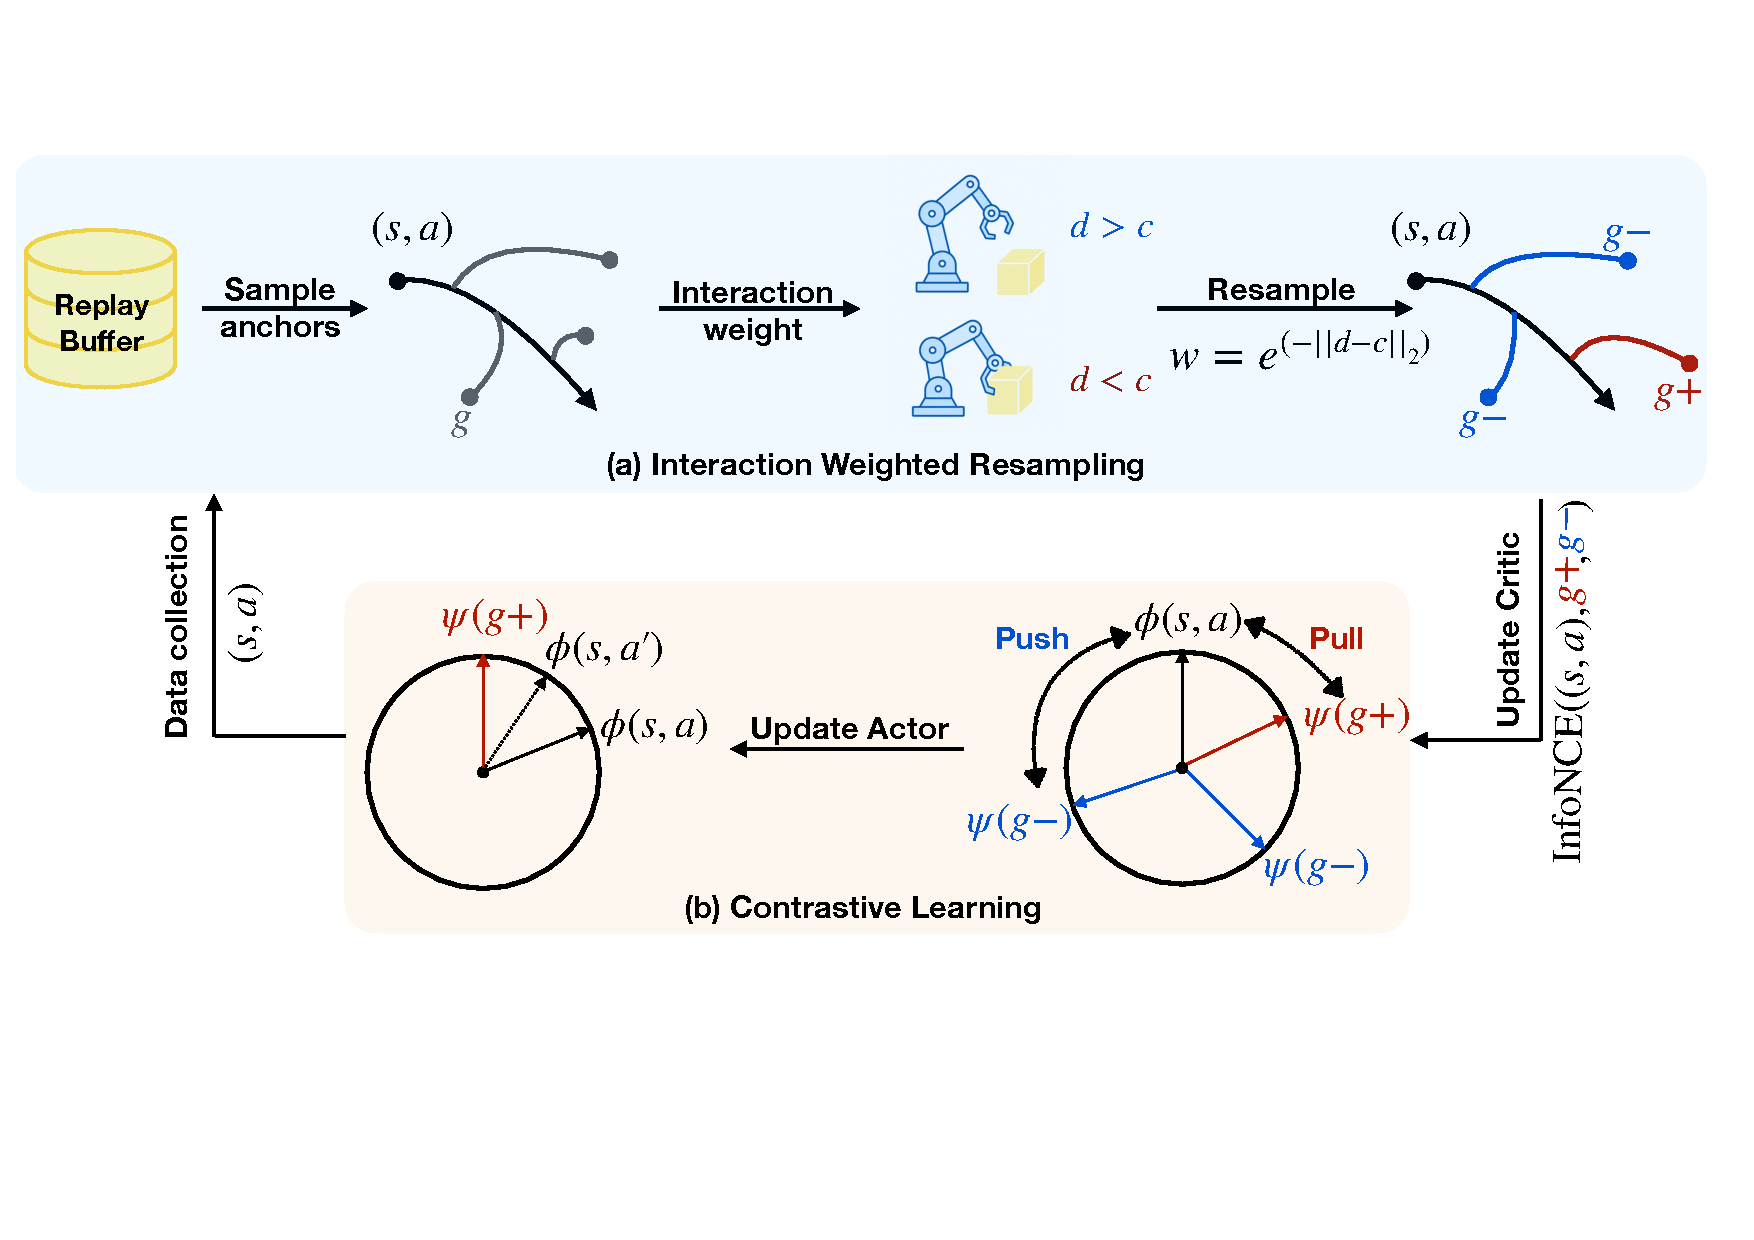
\includegraphics[width=1.0\linewidth]{figure/fig2.pdf}
    \caption{\textbf{Overview of the learning framework}. (a) IWR samples anchor state-action pairs from the replay buffer and reweights candidate future goals by their proximity to the interaction threshold, increasing the chance of selecting interaction-relevant positives. 
(b) The resampled positives and replay-marginal negatives are used in the standard CRL critic update. The learned energy then updates the actor, whose new rollouts are added back to the replay buffer.}
    \label{fig:method}
    \vspace{-.5cm}
\end{figure}
%To address these challenges,  we propose {Interaction-Weighted Resampling (IWR)}, aiming to emphasize contrastive-energy updates on the interaction part.
To address the weak identification of interactions under standard CRL sampling, we propose \emph{Interaction-Weighted Resampling} (IWR). The goal of IWR is to shift the effective contrastive training distribution toward interaction-centered futures, while leaving the CRL critic objective unchanged.

For an anchor transition $x_t=(s_t,a_t)$, we consider a set of candidate future goals $g_k=s_{t+k}$ from the same trajectory. Let $u_{p,t+k}$ and $y_{p,t+k}$ denote the positions of the actuated factor and target factor at the candidate future time $t+k$, respectively. We define their distance as
\begin{equation*}
    d_{t+k}=\|u_{p,t+k}-y_{p,t+k}\|_2 .
\end{equation*}
Let $c$ be a loose interaction threshold, encoding prior knowledge of where interaction is likely to occur, e.g., contact distance between the gripper and object. IWR assigns each candidate a future soft interaction weight:
\begin{equation}
    w_k
    =
    \epsilon
    +
    \exp\left(
        -\frac{||d_{t+k}-c||_2}{2\sigma^2}
    \right),
    \label{eq:iwr}
\end{equation}
where $\epsilon>0$ preserves global coverage and $\sigma$ controls the width of the interaction window. 
%For each sampled transition $(u,y,a)$, denote the position of the actuated factor as $u_p$ and the position of the target factor as $y_p$.
%Let the distance be $d=\|u_p-y_p\|_2$, where $\|\cdot \|_2$ denotes $L_2$ distance obtained from state or visual inputs.
%Denote the interaction-threshold heuristic by $c$, a loose constant that encodes prior knowledge about where interactions are most likely to occur.
%With a small noise term $\epsilon$ and the emphasis power $\sigma$, we calculate the interaction-weighting label $w$ as:
%\begin{equation}
%    w = \epsilon + \frac{1}{\sigma}\exp(-\|d-c\|_2)
%\label{eq:iwr}
%\end{equation}
%Figure~\ref{fig:method} shows the whole learning pipeline of our algorithm.
%We first sample an anchor $(s,a)$ and multiple future goals $g$ from the replay buffer.
%Next, IWR calculates the sampling weight of each future goal using Eq.~\ref{eq:iwr}.
Figure~\ref{fig:method} summarizes the learning pipeline. We first sample anchors \((s,a)\) from the replay buffer and collect candidate future goals from the same trajectory. IWR computes the interaction weights in Eq.~\ref{eq:iwr} and resamples positive futures toward likely interaction regions. The resampled positives are then used in the standard CRL critic objective in Eq.~\ref{eq:sgcrl-critic-objective}. The actor is updated by maximizing the learned goal-reaching energy, and the updated policy collects new transitions into the replay buffer, forming a self-improving loop. Then, the method follows the standard Contrastive RL pipeline: it trains the critic with Eq.~\ref{eq:sgcrl-critic-objective} and updates the actor policy by $\pi = \text{argmax}_a E(s,a,g)$.
Finally, the updated policy collects new transitions in the replay buffer. 
Thus, \methodshort{} focuses the sampling distribution of contrastive updates towards mode-switching regions to improve the modeling of this region. We describe the tighter link between \methodshort{} and Proposition~\ref{prop:endpoint-energy-error} in Appendix~\ref{app:iwr_details}.

% Importantly, IWR does not change the CRL loss or its energy landscape directly. Instead, it changes the effective sampling distribution of contrastive updates. This provides an inductive bias toward mode-switching regions, giving more critic updates to interaction-relevant transitions rather than to easy passive motion or object-reaching behavior. In terms of our analysis (Section~\ref{sec: analysis}), IWR increases the probability that sampled positive futures cross the interaction bridge near the latent interaction time \(\tau_t\). Such samples expose the interaction shift directly, instead of observing it only after long passive propagation through powers of \(A_0\). This also connects to Proposition~\ref{prop:endpoint-energy-error} as increasing the coverage of interaction-centered samples reduces the error contribution from the interaction residual. Exact bridge samples provide direct supervision for the piecewise jump term, while the soft weighting in Eq.~\ref{eq:iwr} also covers nearby positives and reduces error accumulation from repeatedly propagating the interaction signal through \(A_0^k\).
% Consequently, IWR reduces the passive bias of ordinary future sampling and improves the conditioning of interaction-relevant representation learning.


%We preserve the CRL loss landscape while adding an inductive bias that yields more updates on the interaction part, rather than on easy-to-learn object-reaching behavior or uncontrollable passive target-object motion.
%Intuitively, based on the analysis of intrinsic reward \cite{bastankhah2026demystifying}, our paradigm shifts intrinsic reward-driven exploration from ``moving the object to the future'' to ``learning how to control the object to move to the future.''
%Based on Proposition~\ref{prop:endpoint-energy-error}, a higher coverage of the interaction term would control the error bound $|\widehat{E}_k - E_k|$
%. On the one hand, exact interaction positives would help estimate the piecewise jump transfer by controlling the error bound of $\|e\|$.
%On the other hand, soft weighting label would sample positives close to the interaction point. Then we could reduce the accumulation of errors from the exponential iteration of $\|A_0^k\|$.
%As a result, interaction control would be more consistent and robust.



